\laatikko[Jaollisuus]{
	\textbf{Määritelmä 1}
	Kokonaisluku $a$ on jaollinen kokonaisluvulla $b \neq 0$, jos on olemassa kokonaisluku $c$ niin, että $a = b \cdot c$. Tällöin sanotaan myös, että $b$ on $a$:n \termi{tekijä}{tekijä}. Tällöin voidaan merkitä $b|a$, joka luetaan ''$b$ jakaa$a$:n'' tai ''$b$ on $a$:n tekijä''.

	\vspace*{24pt}

	\textbf{Määritelmä 2}
	Luku $a$ on jaollinen luvulla $b \neq 0$, mikäli $\frac{a}{b}$ on kokonaisluku.
	%myöhemminhuomautus, että jaollisuudesta puhutaan vain kokonaislukujen yhteydessä, ei esim- rationaalilukujen
	Määritelmät ovat yhtäpitäviä.
}
    
\begin{esimerkki}
	\alakohdat{
		§ Luku $-12$ on jaollinen luvulla $3$, sillä $-12 = 3 \cdot (-4)$.
		§ $-12$ ei ole jaollinen luvulla $5$, sillä ei ole kokonaislukua, joka kerrottuna viidellä olisi $12$.
	}
\end{esimerkki}
   
\begin{center}
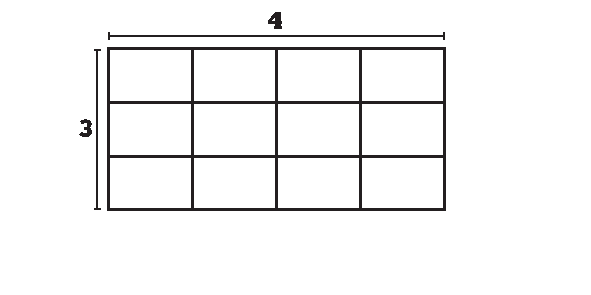
\includegraphics[scale=0.85]{pictures/Kuva2-4-3x4.pdf}
\end{center}
    
Kaikki luvut ovat jaollisia itsellään ja luvulla $1$. Esimerkiksi $7=7 \cdot 1=1 \cdot 7$, joten $7$ on jaollinen luvuilla $1$ ja $7$.
    
\laatikko[Alkuluku]{
	\termi{alkuluku}{Alkuluku} on lukua yksi suurempi luonnollinen luku, joka ei ole jaollinen muilla positiivisilla kokonaisluvuilla kuin luvulla $1$ ja itsellään.
}

\begin{esimerkki}
	\alakohdat{
		§ Luvut $2$, $3$, $5$, $7$, $11$, $13$, $17$ ja $19$ ovat alkulukuja.
		§ Luku $18$ ei ole alkuluku, koska se on jaollinen esimerkiksi luvulla $9$.
		§ Mikään negatiivinen luku ei voi olla alkuluku, koska jokainen negatiivinen luku $-a$ voidaan kirjoittaa tulona $-1\cdot a$.
	}
\end{esimerkki}

Jos luvun tekijä on alkuluku, sitä kutsutaan \termi{alkutekijä}{alkutekijäksi}.

% \begin{esimerkki}
% 	\alakohdat{
% 		§ 
% 	
% 	}
% \end{esimerkki}

\laatikko[Aritmetiikan peruslause]{
Jokainen ykköstä suurempi kokonaisluku voidaan esittää (termien järjestystä lukuunottamatta) yksikäsitteisesti alkulukujen tulona. Jokainen yhtä suurempi kokonaisluku voidaan jakaa alkutekijöihin (termien järjestystä lukuunottamatta) yksikäsitteisellä tavalla.
}

Aritmetiikan peruslause todistetaan kurssilla Logiikka ja lukuteoria. %FIXME: kurssiviittaus
    
Esimerkiksi luku $84$ voidaan kirjoittaa muodossa $2\cdot 2\cdot 3\cdot 7$. Havaitaan, että $2$, $3$, ja $7$ ovat kaikki alkulukuja. Aritmetiikan peruslauseen nojalla tiedetään, että tämä on ainoa tapa kirjoittaa $84$ alkulukujen tulona -- mahdollista kerrottavien termien järjestyksen vaihtoa lukuunottamatta.

Luvun alkutekijät voi löytää etsimällä luvulle ensin jonkin esityksen kahden luvun tulona. Näiden kahden luvun ei tarvitse olla alkulukuja. Sen jälkeen sama toistetaan näille kahdelle luvulle ja edelleen aina uusille luvuille, kunnes jäljellä on vain alkulukuja.

% \begin{esimerkki}
% 	\alakohdat{
% 		§ 
% 	
% 	}
% \end{esimerkki}


